\section{Question 4}

\begin{question}
    Use \MATLAB's \verb+csape+ function from the Curve Fitting Toolbox with the end condition \verb+`variational'+ to interpolate the function $f(x) = 2\cos x$ on $[0,2\pi]$ in $n=5$ even subintervals with a natural cubic spline. Interpolate the same data with the \verb+`not-a-knot'+ end condition (or the \verb+spline+ function) and compare the results.
\end{question}

\subsection{Part a}

\begin{question}
    Plot both interpolating polynomials and $f(x)$ on the same plot over $[0,2\pi]$. You'll need to use \verb+fnplt+ to plot the result of \verb+csape+
\end{question}

\begin{answer}
    In \MATLAB, I used the following code to do the interpolating and plotting:
    \begin{verbatim}
        x = linspace(0,2*pi,5);
        y = 2*cos(x);
        xQ = linspace(0,2*pi,50000);
        f = 2*cos(xQ);
        % Using the csape function with end condition of 'variational'
        P1 = csape(x,y,'variational');
        % Using the csape function with end condition of 'not-a-knot'
        P2 = csape(x,y,'not-a-knot');
        % 4(a)
        figure
        hold on
        fnplt(P1,'b--');
        fnplt(P2,'c--');
        plot(x,y,'ro','MarkerFaceColor','r');
        plot(xQ,f,'k','LineWidth',2.0);
        hold off
        legend ''variational'' ...
        ''not-a-knot'' 'f(x)' ...
            Location SouthEast
    \end{verbatim}
    Then, I got a result as shown in the Figure \ref{fig:fig7}.
    \begin{figure}[H]
        \centering
        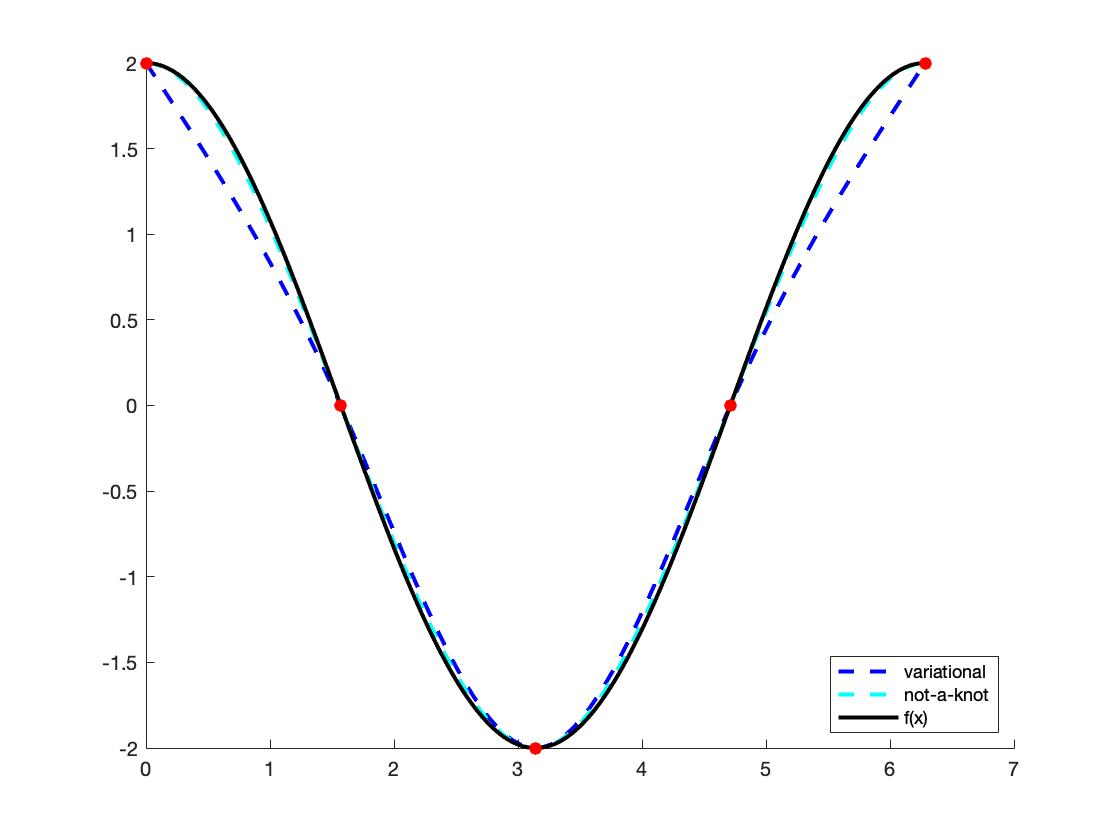
\includegraphics[width=0.9\textwidth]{Figure 7.jpg}
        \caption{\label{fig:fig7}Plot of both interpolating polynomials and f(x) over $2\pi$}
    \end{figure}
\end{answer}

\subsection{Part b}

\begin{question}
    Which approximation is better? Why is the one you chose better? Discuss in a few sentences, and mention where the approximations are different, and what about $f(x)$ makes them different there.
\end{question}

\begin{answer}
    From the plot in the Figure \ref{fig:fig7}, the end condition of \verb+not-a-knot+ gives a better approximation. To be more specific, the \verb+not-a-knot+'s approximation is better at the end points around $x = 0$ and $x = 2\pi$ than the approximation of the \verb+variational+. The reason behind this might be that the end condition \verb+not-a-knot+ uses the third-order derivative to do the interpolating, which makes the curve smoother, which is closed in this case since $2\cos{(x)}$ is more curved at the ends of the interval $[0,2\pi]$. However, the end condition \verb+variational+ uses the natural boundary condition, which only involves the second-order derivatives, this makes it less smooth than the curve interpolated by the \verb+not-a-knot+ condition.
\end{answer}